\documentclass{beamer}

\mode<presentation>
{
  \usetheme{Frankfurt}
  \setbeamercovered{transparent}
  \useoutertheme{tree}
  \useinnertheme{rounded}
}

\usepackage[spanish]{babel}
\usepackage[utf8]{inputenc}

\usepackage{times}
\usepackage[T1]{fontenc}

% Redefinicion de teorema, definicion, ejemplo
\newtheorem{teorema}{Teorema}
\newtheorem{definicion}{Definición}
\newtheorem{ejemplo}{Ejemplo}

\hypersetup{colorlinks=true,linkcolor=red}

\title{Desarrollo colectivo en Turpial}
\author[Wil Alvarez \and Milton Mazzarri]{Wil Alvarez \texttt{<wil.alvarez@gmail.com>} \\
Milton Mazzarri \texttt{<milmazz@gmail.com>}
}
\institute[Cayapa Canaima]{3ra. Cayapa Canaima}
\date{Marzo, 2010}

\subject{Desarrollo colectivo en Turpial}

\pgfdeclareimage[height=1cm]{turpial-logo}{pics/turpial-logo}
\logo{\pgfuseimage{turpial-logo}}

 \AtBeginSubsection[]
{
  \begin{frame}<beamer>[allowframebreaks]{Contenido}
    \tableofcontents[currentsection,currentsubsection]
  \end{frame}
}

% If you wish to uncover everything in a step-wise fashion, uncomment
% the following command: 

%\beamerdefaultoverlayspecification{<+->}

\begin{document}

\begin{frame}
    \titlepage
\end{frame}

\begin{frame}[allowframebreaks]{Contenido}
    \tableofcontents[pausesections]
\end{frame}

\section{Historia}

\frame{
    \frametitle{Historia}

    \begin{itemize}
    \item \emph{Adobe AIR} solo funciona en \textbf{GNOME}, \textbf{KDE}.
    \item Poca integración con el escritorio.
    \item Los clientes \textbf{GTK} existentes para la época eran pobres.
    \item Los clientes \emph{Adobe AIR} son funcionales pero \emph{NO} libres.
    \item Ninguno cubría las expectativas.
    \item La motivación de otros compañeros a iniciar el desarrollo.
    \end{itemize}
}

\frame{
    \frametitle{Clientes de Twitter disponibles}
    \begin{center}
    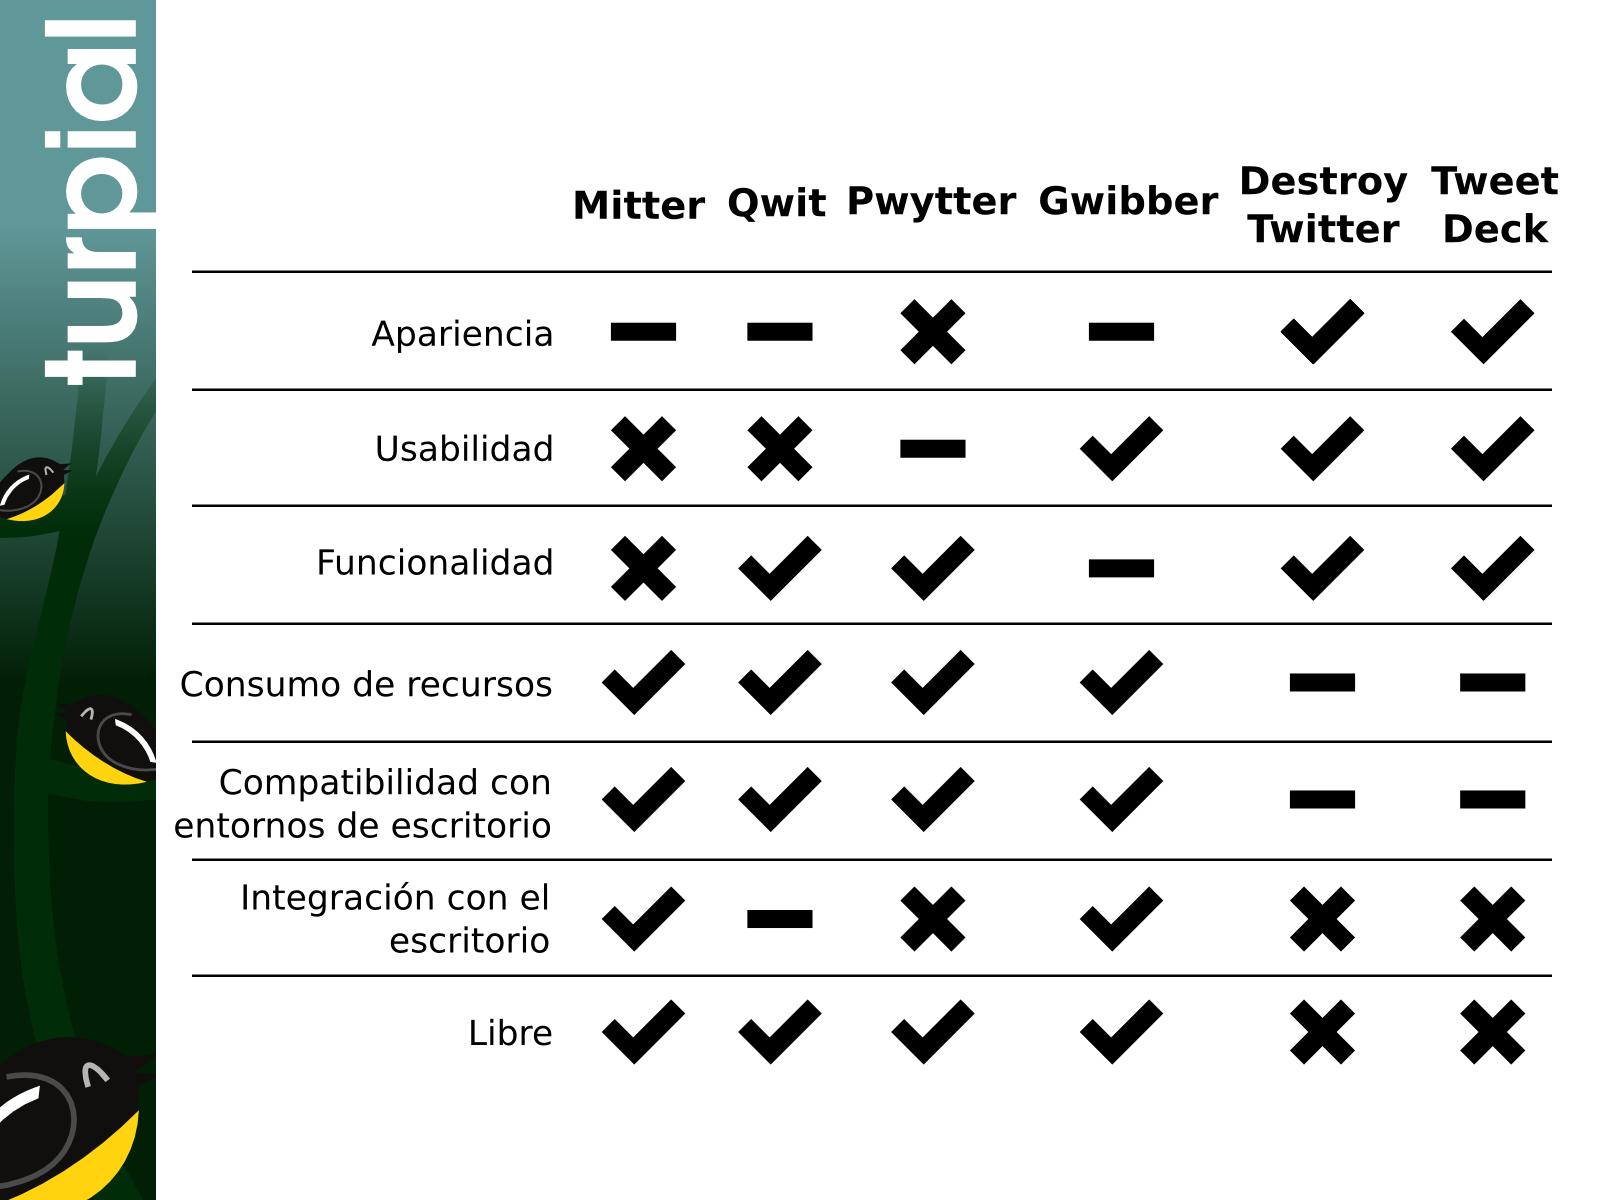
\includegraphics[height=5cm]{pics/otros-clientes-twitter.png}
    \end{center}
}

\section{Visión}
\frame{
    \frametitle{Visión}

    \begin{itemize}
        \item Cliente alternativo para Twitter con múltiples interfaces.
        \item Bajo consumo de recursos.
        \item Estar integrado en el escritorio del usuario sin renunciar a ninguna funcionalidad.
        \item Poder ejecutarse en escritorios ligeros como Fluxbox, OpenBox, entre otros.
        \item Ser accesible para personas con discapacidad.
    \end{itemize}
}

\frame{
    \frametitle{Características}

    \begin{center}
    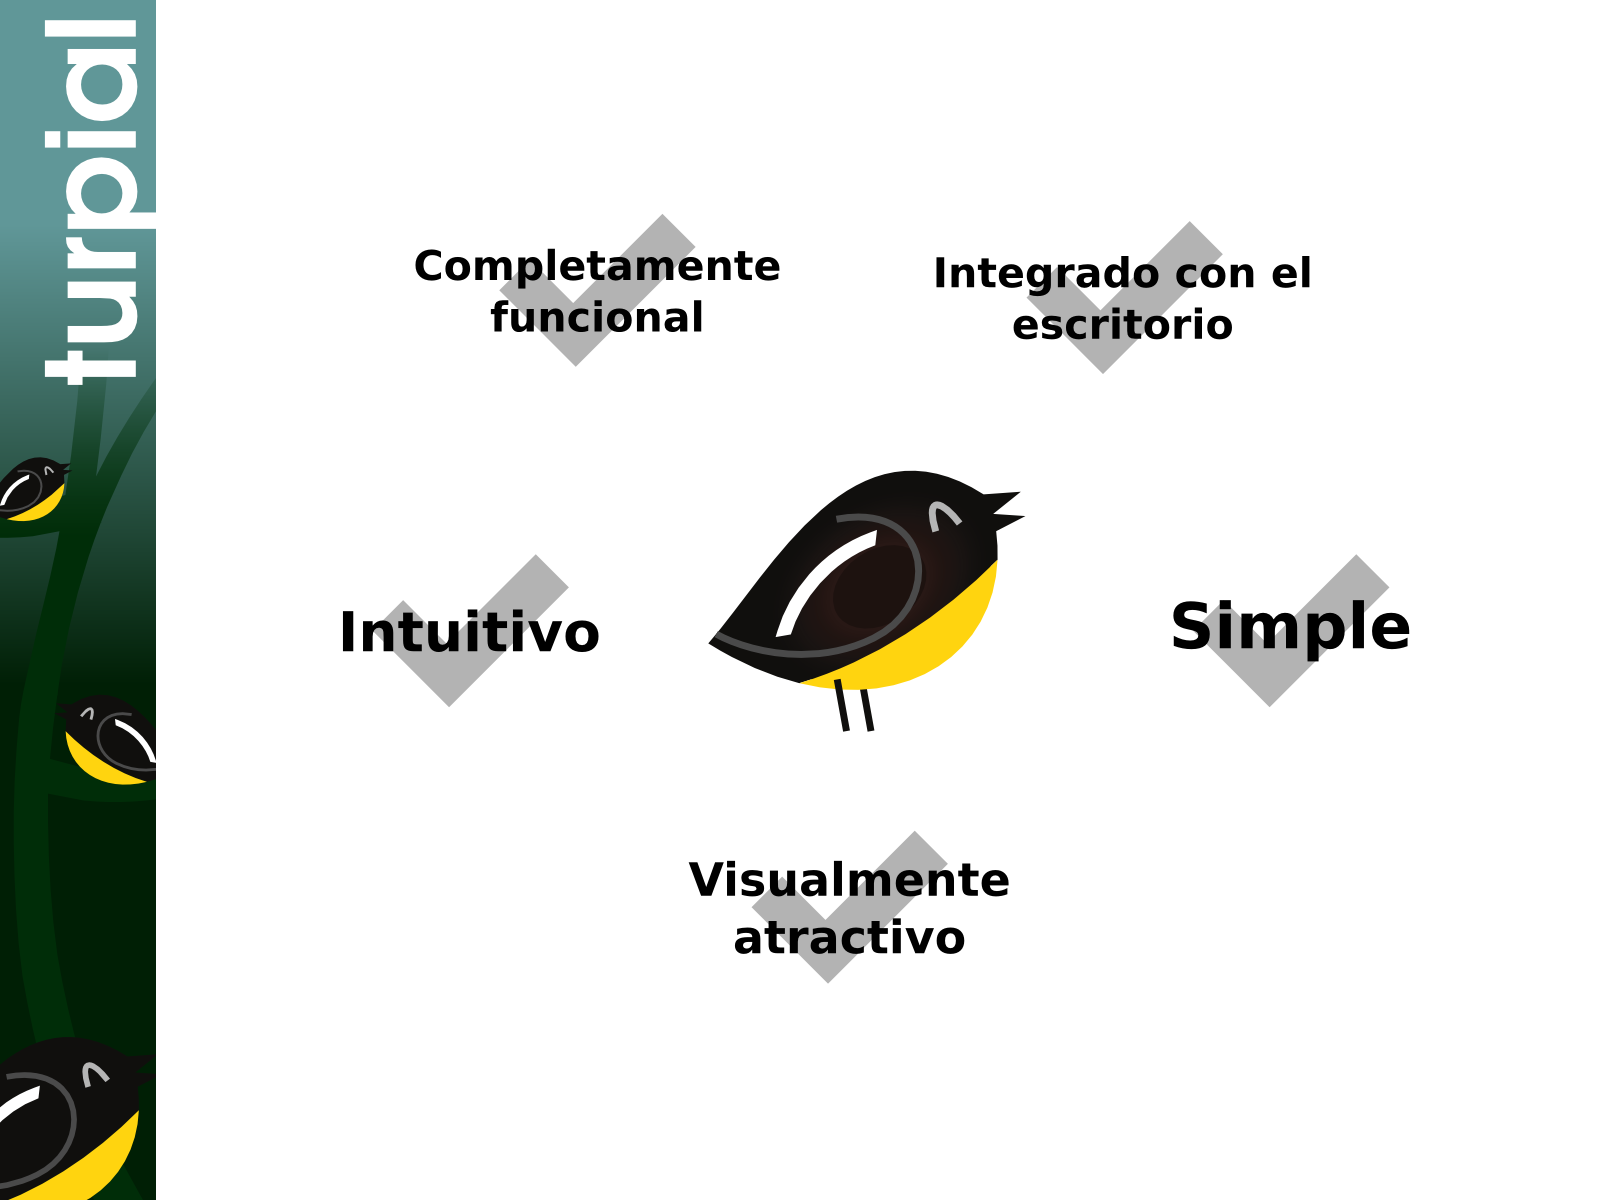
\includegraphics[height=5cm]{pics/caracteristicas.png}
    \end{center}
}

\section{Conociendo Turpial}

\subsection{Tecnologías}
\frame{
    \frametitle{Tecnologías usadas}

    \begin{center}
    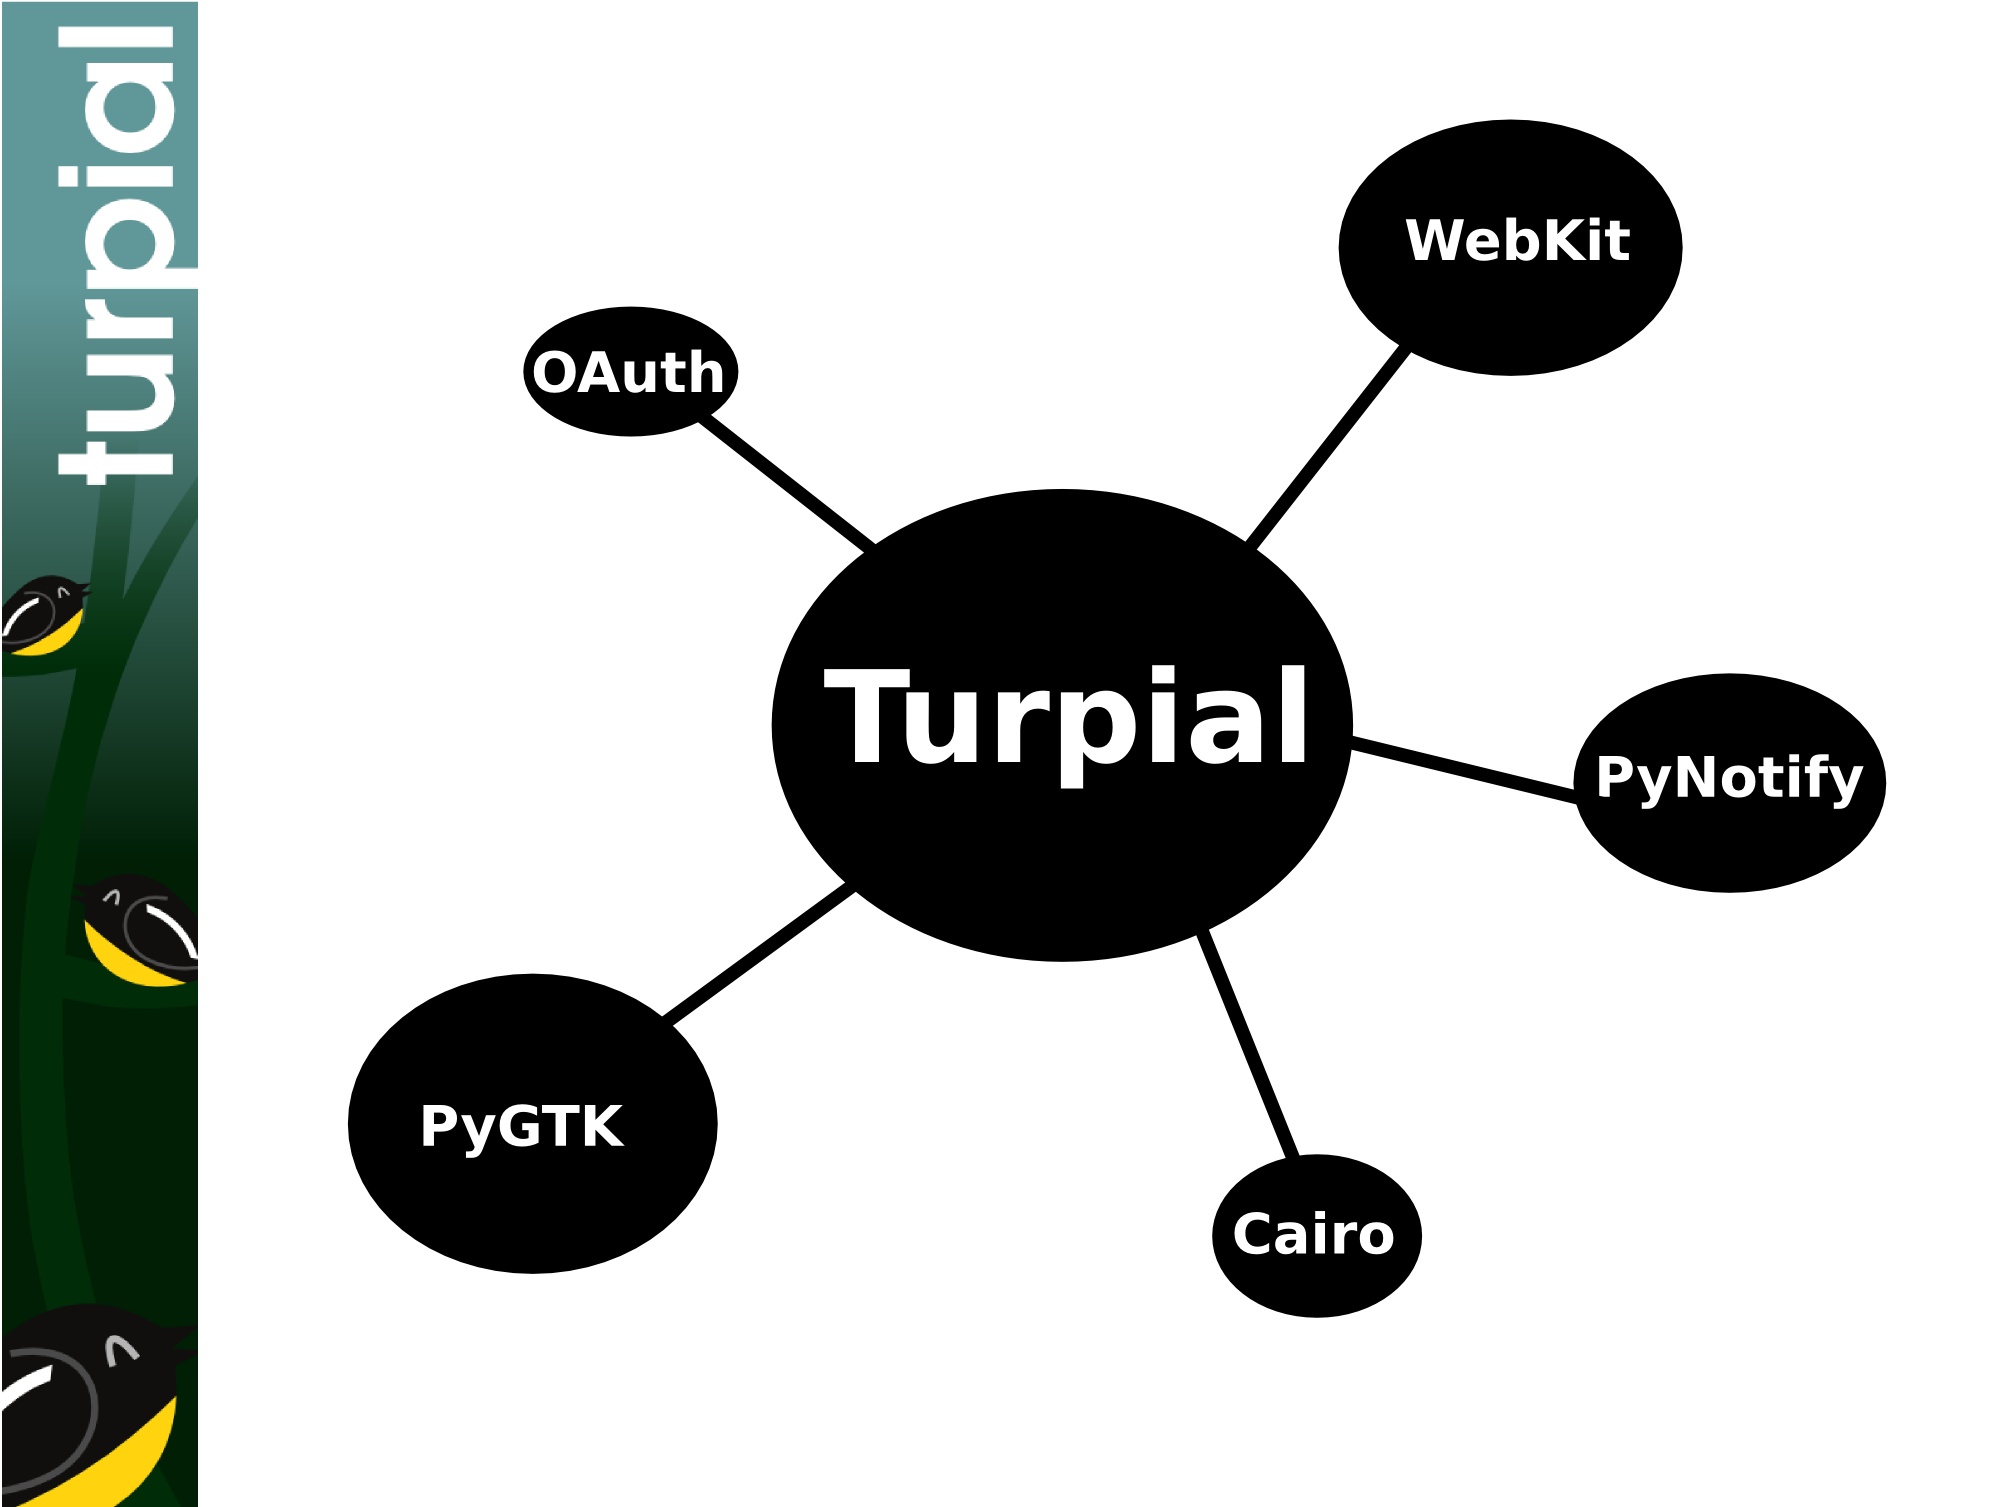
\includegraphics[height=5cm]{pics/tecnologias.png}
    \end{center}
}

\subsection{Evolución}

\frame{

    \frametitle{Turpial 1.0}

    \begin{center}
    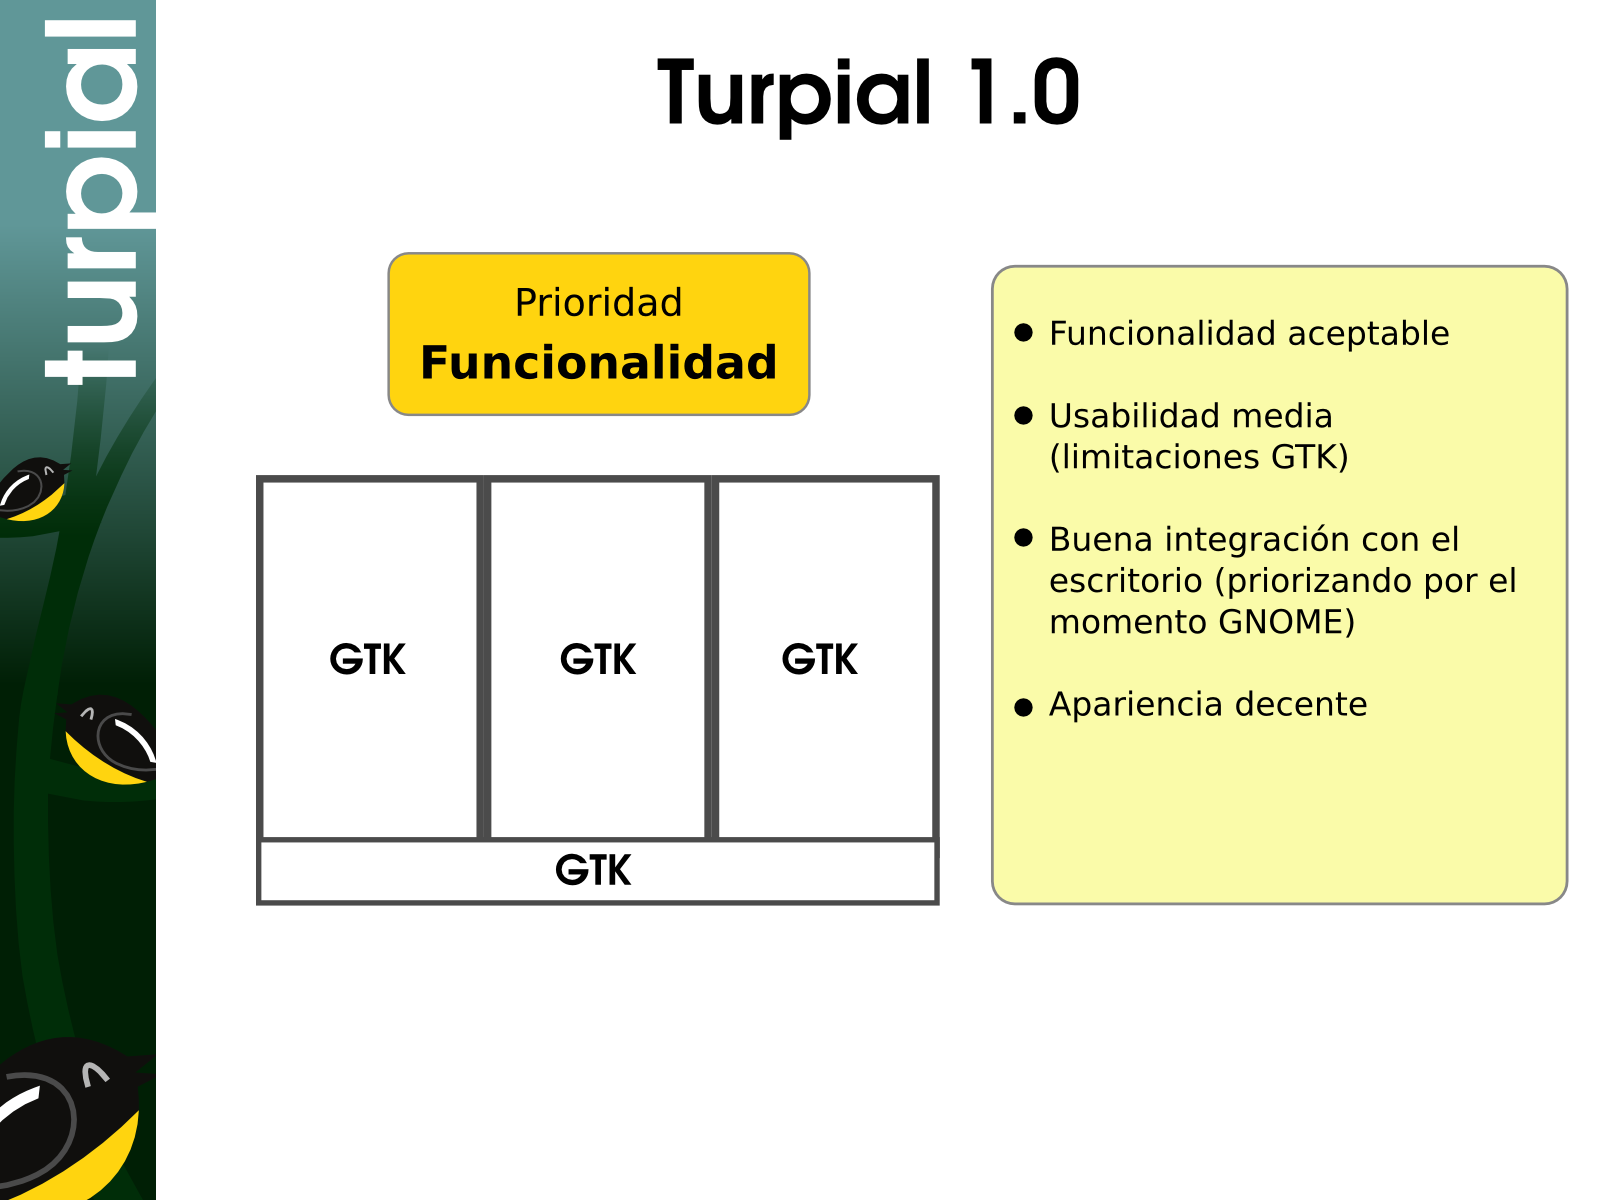
\includegraphics[height=5cm]{pics/v1_0.png}
    \end{center}
}

\frame{

    \frametitle{Turpial 1.5}

    \begin{center}
    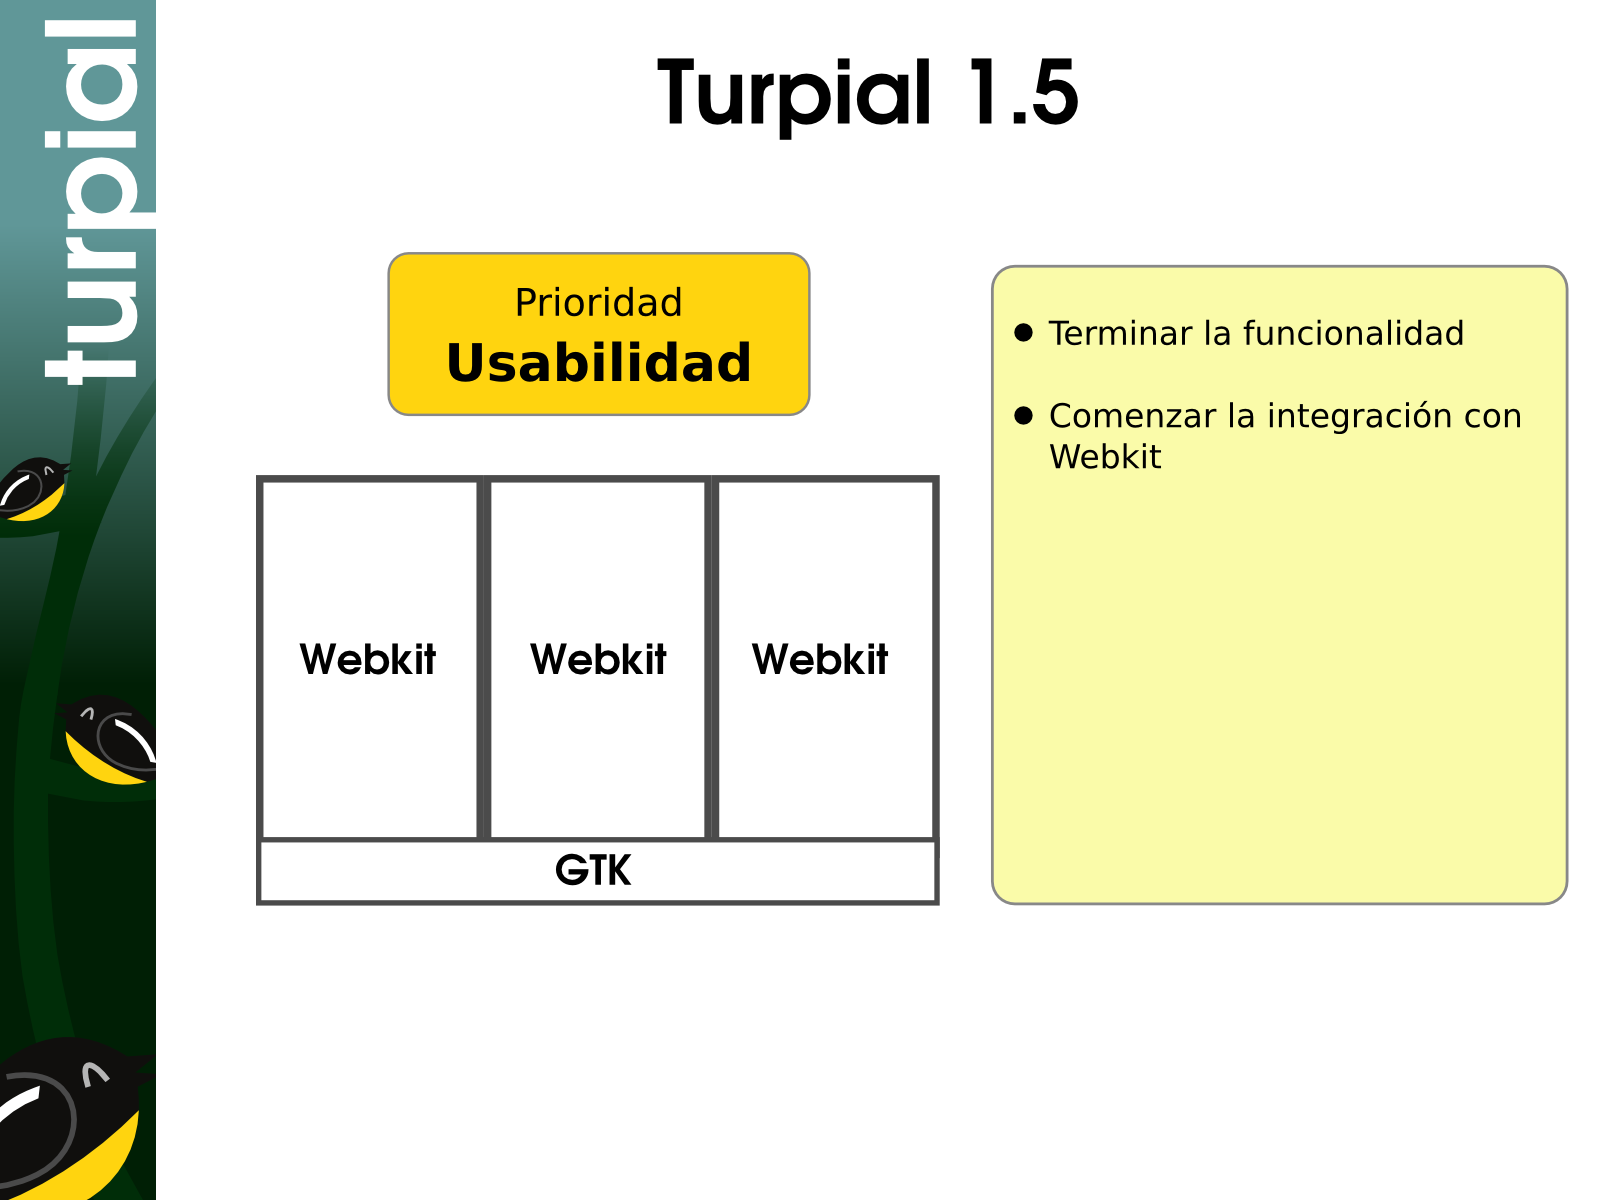
\includegraphics[height=5cm]{pics/v1_5.png}
    \end{center}
}

\frame{

    \frametitle{Turpial 2.0}

    \begin{center}
    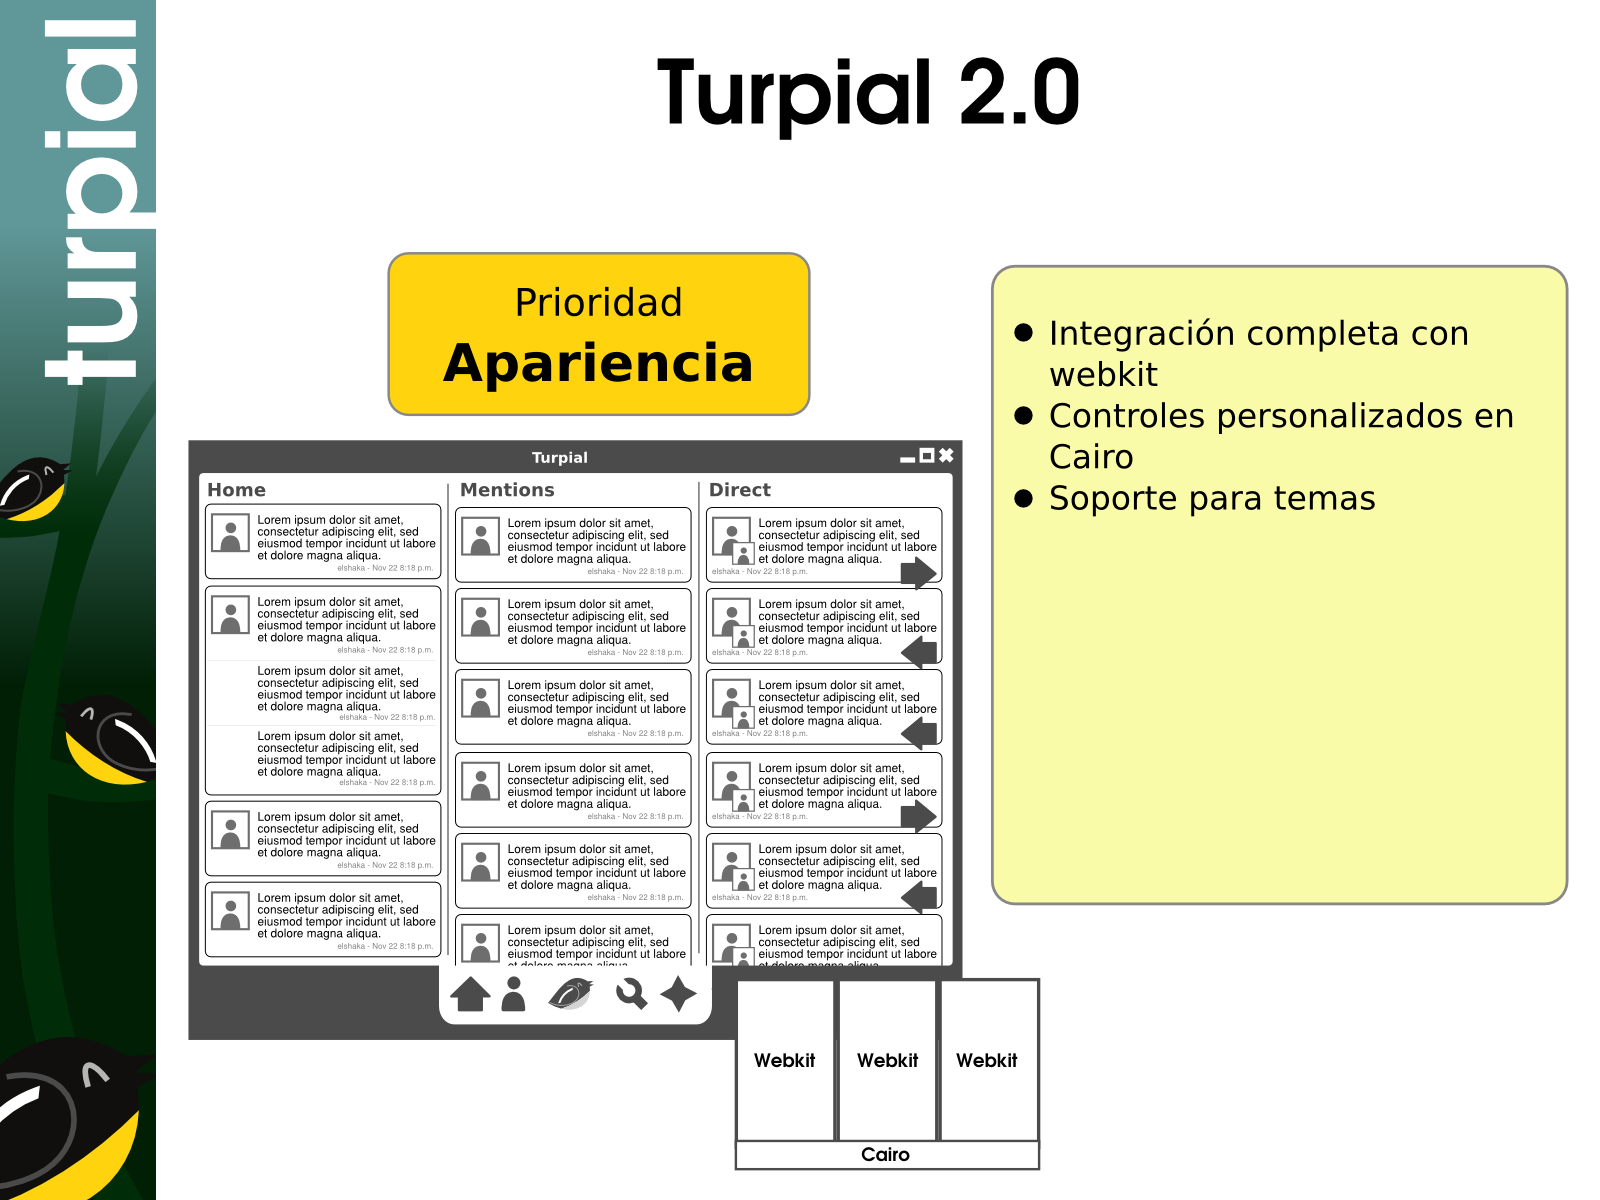
\includegraphics[height=5cm]{pics/v2_0.png}
    \end{center}
}

\subsection{Modelo MVC}

\frame{
    \frametitle{Modelo MVC en Turpial}

    \begin{center}
    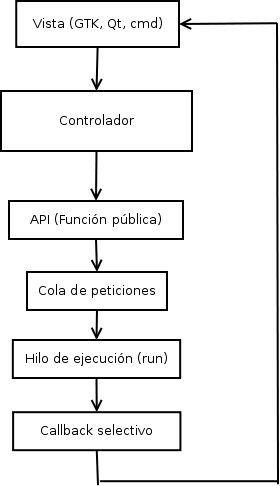
\includegraphics[height=5.5cm]{pics/api.png}
    \end{center}
}

\begin{frame}[fragile]

\frametitle{Estructura de directorios}

\begin{verbatim}
.
|__ doc
|__ turpial
    |__ api
    |   |__ poster
    |__ data
    |   |__ pixmaps
    |   |__ sounds
    |   |__ themes
    |       |__ default
    |__ i18n
    |__ ui
        |__ gtk
        |__ gtk2
\end{verbatim}
\end{frame}

\subsection{Internacionalización}

\begin{frame}[fragile]
\frametitle{Estructura}

\begin{verbatim}
i18n
|__ en
|   |__ LC_MESSAGES
|       |__ messages.mo
|       |__ messages.po
|__ es
|   |__ LC_MESSAGES
|       |__ messages.mo
|       |__ messages.po
\end{verbatim}
\end{frame}

\begin{frame}[fragile]
\frametitle{Localización}

\begin{ejemplo}
\begin{verbatim}
#: turpial/notification.py:58
msgid "new tweet"
msgstr "nuevo tweet"

#: turpial/notification.py:60
msgid "new tweets"
msgstr "nuevos tweets"
\end{verbatim}
\end{ejemplo}
Proyecto Transifex: \url{http://www.transifex.net/projects/p/turpial/c/development/}
\end{frame}

\begin{frame}
\frametitle{Integración PyBabel en Turpial}

\begin{itemize}
    \item \texttt{compile\_catalog}
    \item \texttt{extract\_messages}
    \item \texttt{init\_catalog}
    \item \texttt{update\_catalog}
\end{itemize}
\end{frame}

\subsection{Documentación}

\frametitle{
    \frametitle{Documentación}

    \begin{itemize}
        \item ... 
    \end{itemize}
}

\begin{frame}[fragile]
    \frametitle{Nuestra meta}
\begin{ejemplo}
\tiny
\begin{verbatim}
def fibonacci():
    """
    Return the *Fibonacci number*

    Interesting bits:

    >>> fib = fibonacci()
    >>> fib.next()
    1
    >>> fib.next()
    1
    >>> fib.next()
    2
    >>> [fib.next() for i in range(10)]
    [3, 5, 8, 13, 21, 34, 55, 89, 144, 233]
\end{verbatim}
\end{ejemplo}
\end{frame}

\begin{frame}[fragile]
    \frametitle{Nuestra meta}
\begin{ejemplo}
\tiny
\begin{verbatim}
    :var first_seed: F\ :sub:`0`\  feed seed.
    :type first_seed: int
    :var second_seed: F\ :sub:`1`\  feed seed.
    :type second_seed: int
    :return: Return the `Fibonacci number`_
    :rtype: int

    .. _`Fibonacci number`: http://en.wikipedia.org/wiki/Fibonacci_number
    """
\end{verbatim}
\end{ejemplo}
\end{frame}

\begin{frame}[fragile]
\frametitle{Nuestra meta}

\begin{ejemplo}
\tiny
\begin{verbatim}
    first_seed, second_seed = 0, 1

    while True:
        yield second_seed
        first_seed, second_seed = second_seed, first_seed + second_seed

if __name__ == "__main__":
    import doctest
    doctest.testmod()
\end{verbatim}
\end{ejemplo}

Detalle del código: \url{http://github.com/milmazz/myfibonacci}
\end{frame}

\begin{frame}
\frametitle{Resultados con Sphinx}

\begin{center}
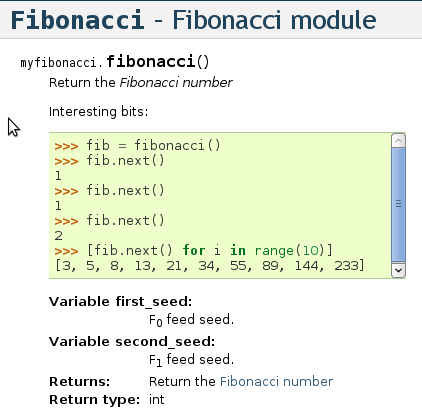
\includegraphics[height=5cm]{pics/sphinx.png}
\end{center}
\end{frame}

\section{Enlaces de interés}

\frame{
    \frametitle{Enlaces de interés}

    \begin{itemize}
    \item \url{http://code.google.com/p/turpial}
    \item \url{http://github.com/satanas/Turpial}
    \item \url{http://github.com/milmazz/Turpial}
    \item \url{http://turpial.org.ve} (Próximamente)
    \end{itemize}
}

\frame{
    \frametitle{Agradecimientos}

    \begin{itemize}
    \item Wil Alvarez (@satanas82) -- Autor y programación.
    \item Eleazar Meza -- Concepto y diseño.
    \item Azrael Arocha -- Pruebas y colaboración.
    \item José Leonel Subero -- Pruebas.
    \item Edwind Contreras -- Pruebas, empaquetado RPM.
    \item William Cabrera -- Pruebas
    \end{itemize}
}

\frame{
    \frametitle{Agradecimientos}

    \begin{itemize}
    \item Marguerite Su (@doublechou) -- Traducción al francés, zh\_CH, zh\_TW.
    \item Flavio Percoco (@flaper87) - Traducción al italiano.
    \item Ana Rangel (@4n1ta) -- Traducción al Noruego.
    \item Solazver Solé -- Traducción al Portugués
    \item Raúl Escalante (@t6435bm) -- Traducción al Alemán.
    \item Milton Mazzarri (@milmazz) -- Programación, traducción al italiano.
    \end{itemize}
}
\end{document}
